\documentclass[letterpaper,12pt]{article}
\usepackage{tabularx} % extra features for tabular environment
\usepackage{amsmath}  % improve math presentation
\usepackage{float}
\usepackage{pdfpages}
\usepackage{graphicx} % takes care of graphic including machinery
\graphicspath{ {./figures/} }
\usepackage[margin=1in,letterpaper]{geometry} % decreases margins
 % takes care of citations
\usepackage[final]{hyperref} % adds hyper links inside the generated pdf file
\hypersetup{
	colorlinks=true,       % false: boxed links; true: colored links
	linkcolor=blue,        % color of internal links
	citecolor=blue,        % color of links to bibliography
	filecolor=magenta,     % color of file links
	urlcolor =blue         
}




\begin{document}

\title{EXPERIMENT\protect\\"LIGHT DEPENDENT RESISTORS AND DISTANCE MEASUREMENTS"}
\author{Prepared by Ahmet Akman 2442366}
\date{\today}
\maketitle
\section*{Objectives}
\begin{itemize}
	\item The Light Dependent Resistor (LDR) component to be characterized.
	\item Distance measurement sensor mechanisms to be indtroduced.
\end{itemize}
\section*{Preliminary Work}
\subsection*{1}
Watch the  videos (provided in Appendix).
\subsection*{2}
Study "Notes on Multimeters".
\subsection*{3}
Light Dependent Resistors (abrevieted as LDRs) are semiconductor based electronic component. An example of an LDR is shown in Figure 1. 
\begin{figure}[H]
	\centering
	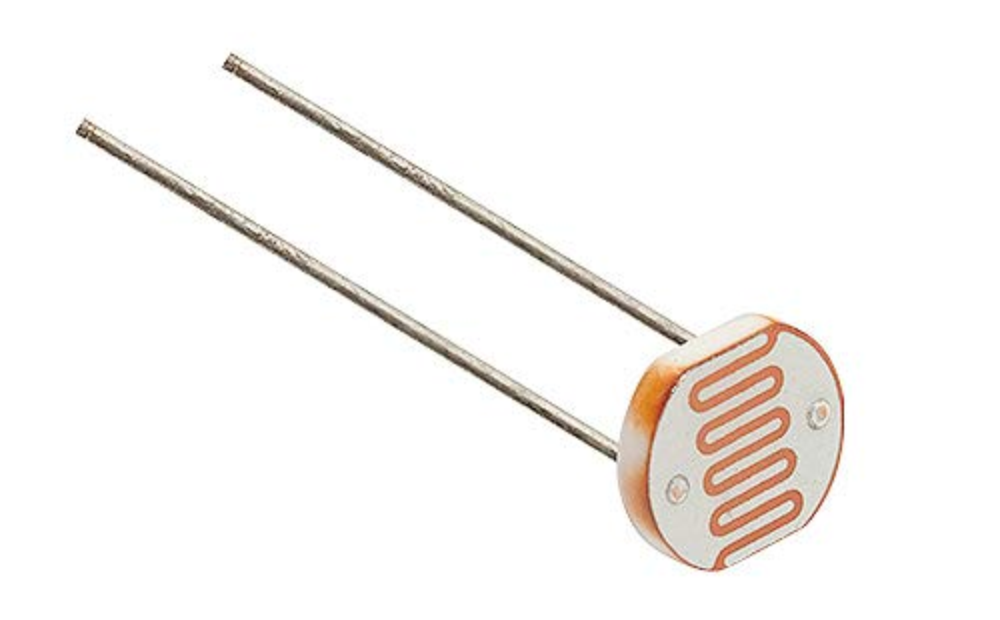
\includegraphics[width=0.5\textwidth]{LDR_photo.png}
	\caption{LDR picture}
\end{figure} 
LDR ,as easily can be inferred from its name, has a variable resistance which depends on the illumination on its surface. So, its resistance is high in dark and low in light. Those resistance values are vastly dependent on the size and the model of the particular LDR. In this step you are required to find an LDR from a manufacturer and from the datasheet provide following informations with necessary plots. You do not need to explain those data, it is enough to provide in the preliminary report with appropriate format.
\begin{itemize}
	\item Sensitive surface area.
	\item Resistance as a function of illumination (with plot).
	\item Spectral response (with plot). 
\end{itemize}   
\subsection*{4}
The schematic symbol of LDR component is given in Figure 2.
\begin{figure}[H]
	\centering
	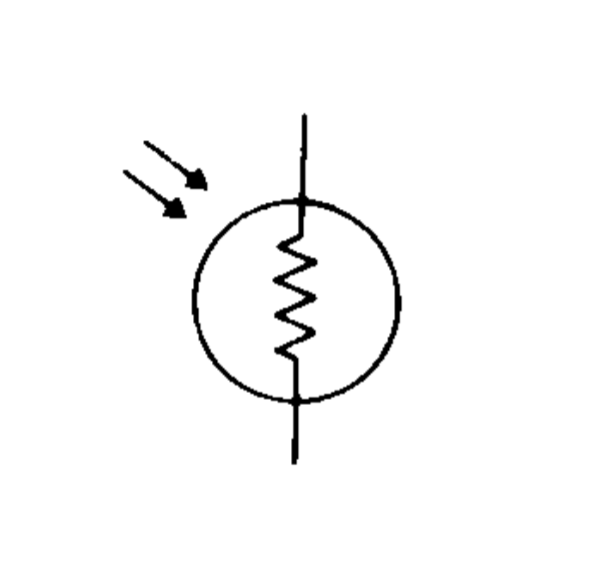
\includegraphics[width=0.5\textwidth]{LDR_symbol.png}
	\caption{LDR schematic symbol}
\end{figure} 
Using this information, briefly describe the functional behavior of the circuit given in Figure 3. (\textbf{Hint:} It would be nice to look back to comparator op-amp setup.)
\begin{figure}[H]
	\centering
	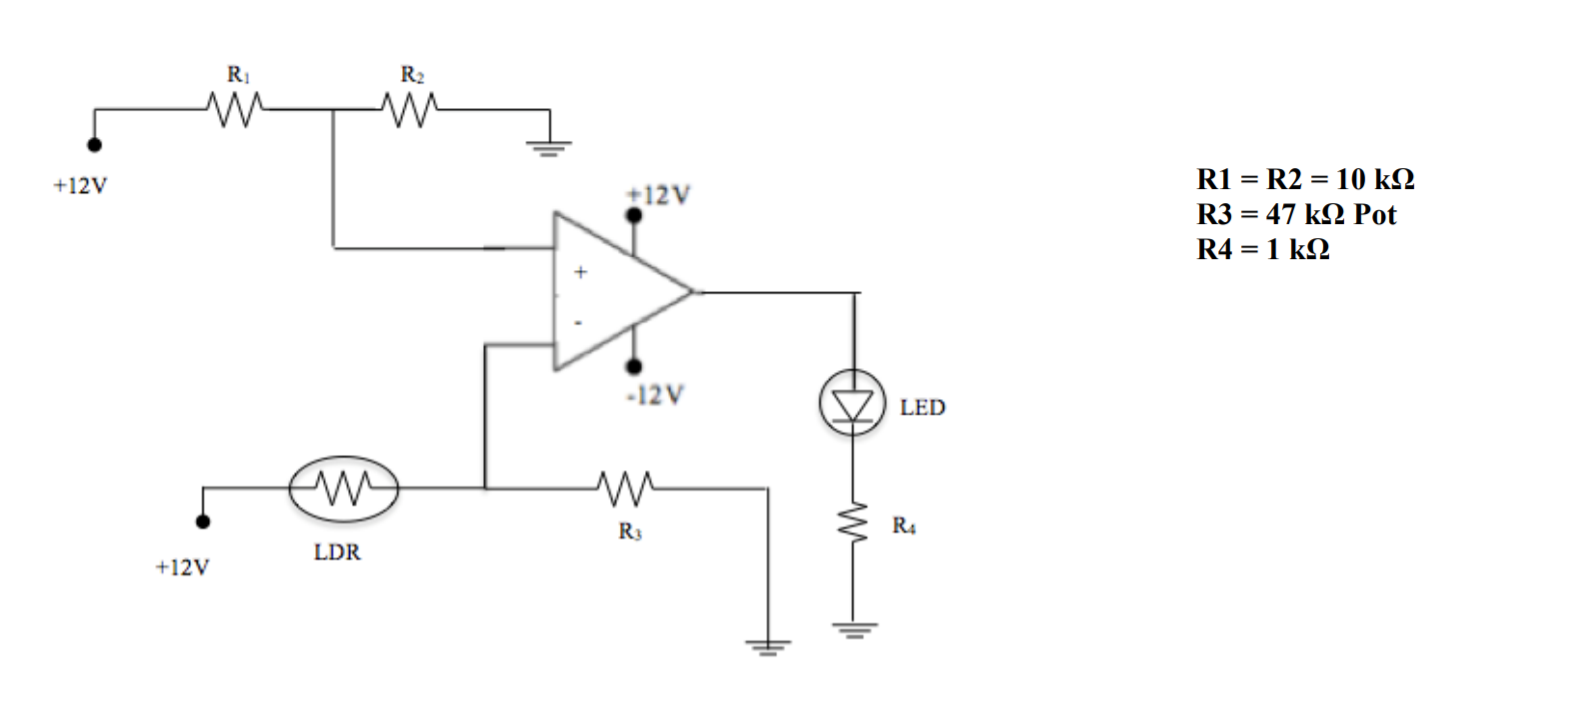
\includegraphics[width=1\textwidth]{darkness.png}
	\caption{A circuit with LDR}
\end{figure} 

\subsection*{5}
For this step you are required to do small research about optical distance sensors. Independent from the experiment, this step is for you to gain an insight on optical distance sensors.
\begin{itemize}
	\item Describe how triangulation measurement method works in \(\sim\) 50-100 words with a credible source. 
	\item Describe how time of flight (ToF) measurement method works in \(\sim\) 50-100 words with a credible source. 
	\item Describe how phase measurement method works in \(\sim\) 50-100 words with a credible source. 
\end{itemize}
\section*{Equipment List}
\begin{itemize}
	\item LDR (Light Dependent Resistor)
	\item Digital Multimeter.
	\item Ruler.
	\item A bright light source like a phone flashlight. (This is expected to be supplied from the student.)
\end{itemize}
\section*{Experimental Work}
Important note - 1: You only need to show your work to the lab assistant for step 2.
\subsection*{Step 1}
Describe the relation between illumination on a surface and the distance of the light source.
\subsection*{Step 2}
In this step you are required to measure the distance of a light source using LDR component. Setup the configuration given in Figure 4 by connecting the probes to the digital multimeter. Adjust the multimeter so that it measures the resistance. 
\begin{figure}[H]
	\centering
	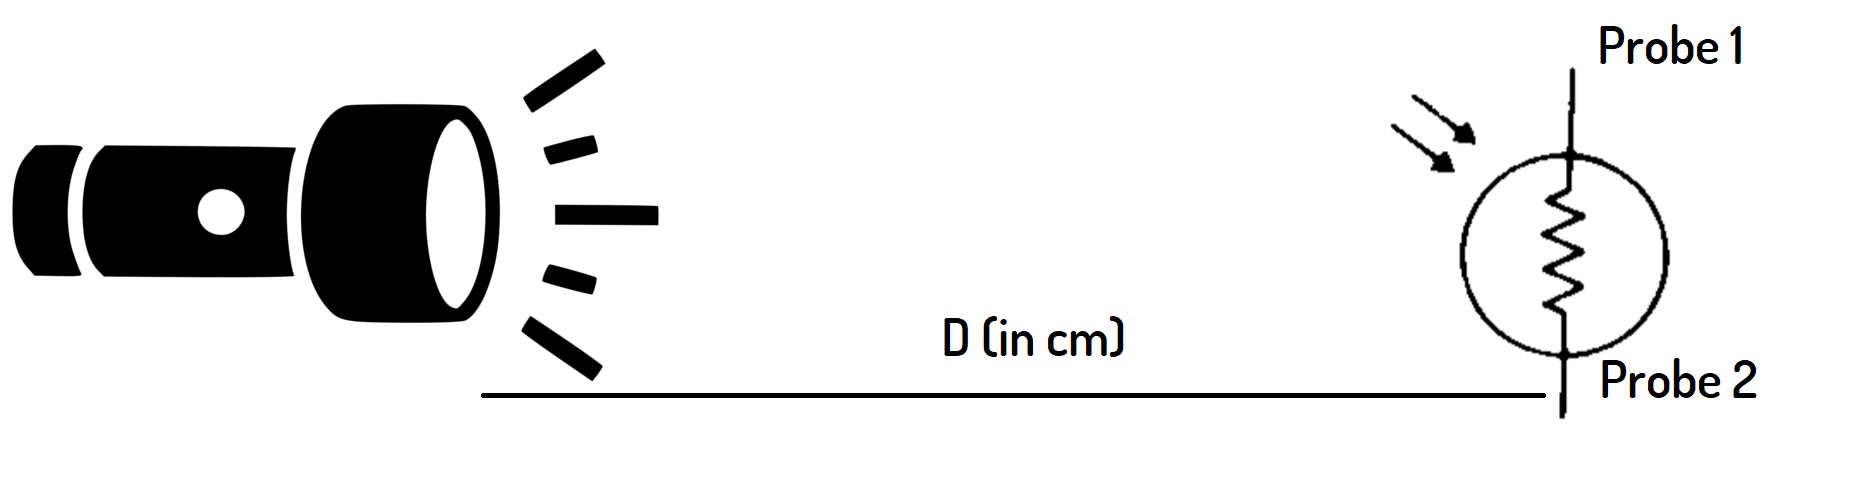
\includegraphics[width=1\textwidth]{setup.png}
	\caption{Simple distance measurement with LDR configuration}
\end{figure}
It is necessary to align the source with  the surface of the LDR for better measurements. Also, pay attention not to  cause the ambient light to fluctuate with shadows.
\subsubsection*{a)}
Using ruler make the distance D as "15 centimeter". Then record the resistance value. Following equation relates distance with the resistance of an LDR ,and prepared by us. X stands for distance in centimeters and you need to find the \(\alpha\) constant to shift curve to the calibrated point by solving the equation with the resistance value you recorded. You may get a help from a calculator.
\[resistance   k\Omega = 0.07847 x^3 -0.3281 x^2 + 0.8929x + \alpha\] 
Plot the resultant equation (in MATLAB). Convey series of arbitrary distances' resistance measurements (at least 5) and record the values. Do not forget to obtain real distance in centimeters with  ruler in order to compare with the results you found. Using the plot you have obtained map the values you recorded to obtain the measured distance. Present  values your found in tabular form in your report. Lastly compare them with the actual ruler measurement and express the deviation by calculation the deviation percentage.\\
\subsection*{b)}
As you practiced in preliminary work, LDR component have various manufacturers and different variations. So, only a base created using another LDR might not be as accurate as map prepared for the particular LDR you use and the ambient light you have. Thus, you are required to measure the resistance with 15 different known (via ruler) distance values and record them. \textbf{Hint:} You can mark where the ruler ends and aliging the same ruler the further distances can be measured. Provide data you have obtained in tabular form and plot (in MATLAB) resistance(in kOhm) vs distance (in cm). Fit an equation to this curve (see Appendix) and plot (in MATLAB). Compare the equation you obtained with the given equation in part a . 
\subsection*{c)}
Map the values you recorded in part a to the plot in part b and calculate the deviations. Then compare the deviation values.
\section*{Step 3} 
Explain the limitations of the method used in Step 2 to measure distance of a light source ,and compare it with the methods you described in the Preliminary Work.
\section*{Appedix I}
MATLAB has the feature of fitting curves to the data. You can fit a curve to a data like given in Figure 5.
\begin{figure}[H]
	\centering
	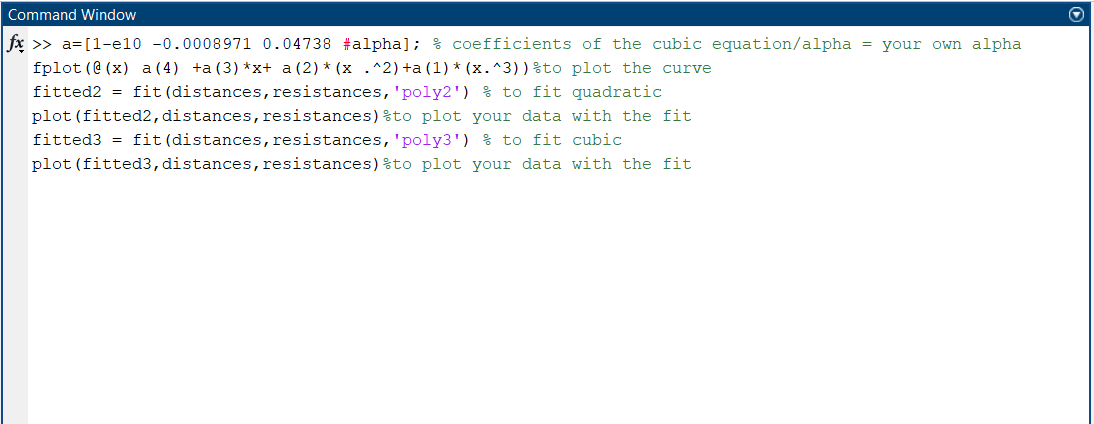
\includegraphics[width=1\textwidth]{appendix.png}
	\caption{MATLAB fit a curve}
\end{figure}
\section*{Appedix II}
The video link is: \url{www.youtube.com}


\end{document}


\begin{table}[H]
	\begin{center}
		\caption{Resistance reading by color code convention.}
		\vspace{2mm}
		\begin{tabular}{||c | c | c||} 
		 \hline
		 Color Order & Value & Tolerance \\ [0.5ex] 
		 \hline\hline
		 Brown / Black / Red / Gold & 1k\( \Omega \) & \( \% \) 5  \\ 
		 \hline
		 Yellow / Violet / Red / Gold & 4.7k\( \Omega \) & \( \% \) 5   \\
		 \hline
		 Brown / Grey / Orange / Gold & 18k\( \Omega \) & \( \% \) 5  \\ [1ex] 
		 \hline
		\end{tabular}
	\end{center}
	\end{table}

\begin{figure}[H]
	\centering
	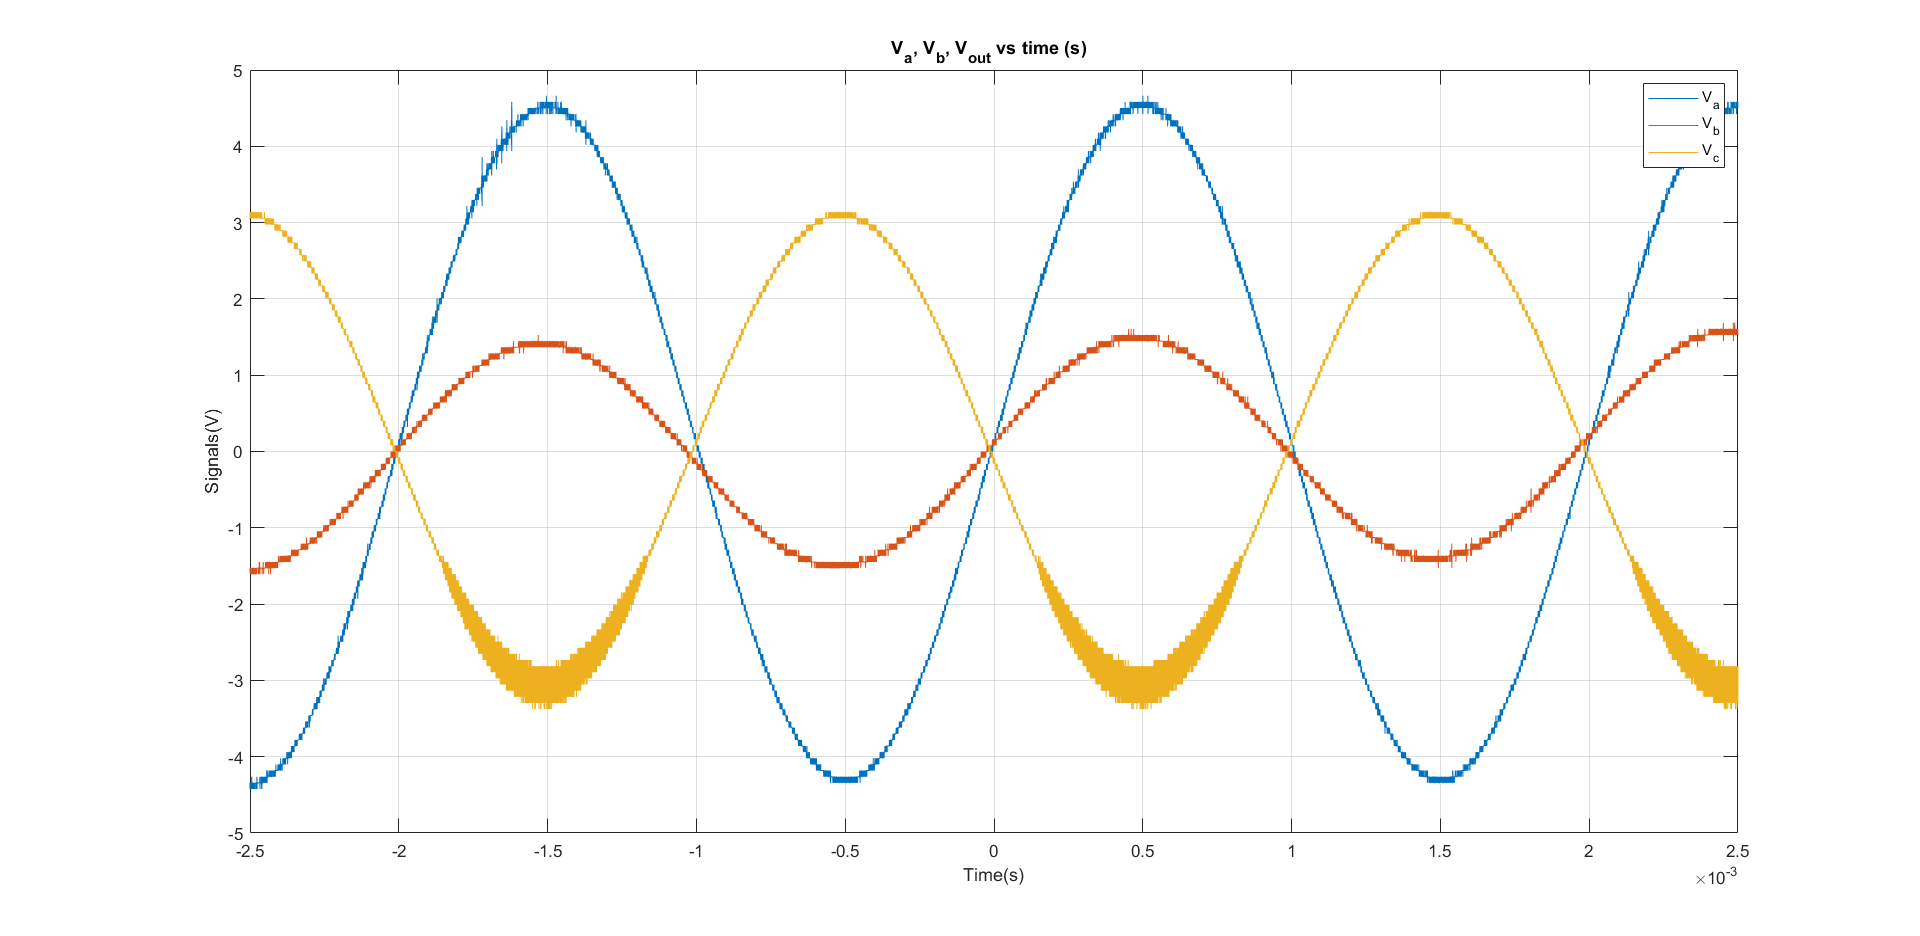
\includegraphics[width=0.6\textwidth]{5.png}
	\caption{Circuit schematic for the step 5}
\end{figure} 

	\begin{figure}[htp] \centering{
		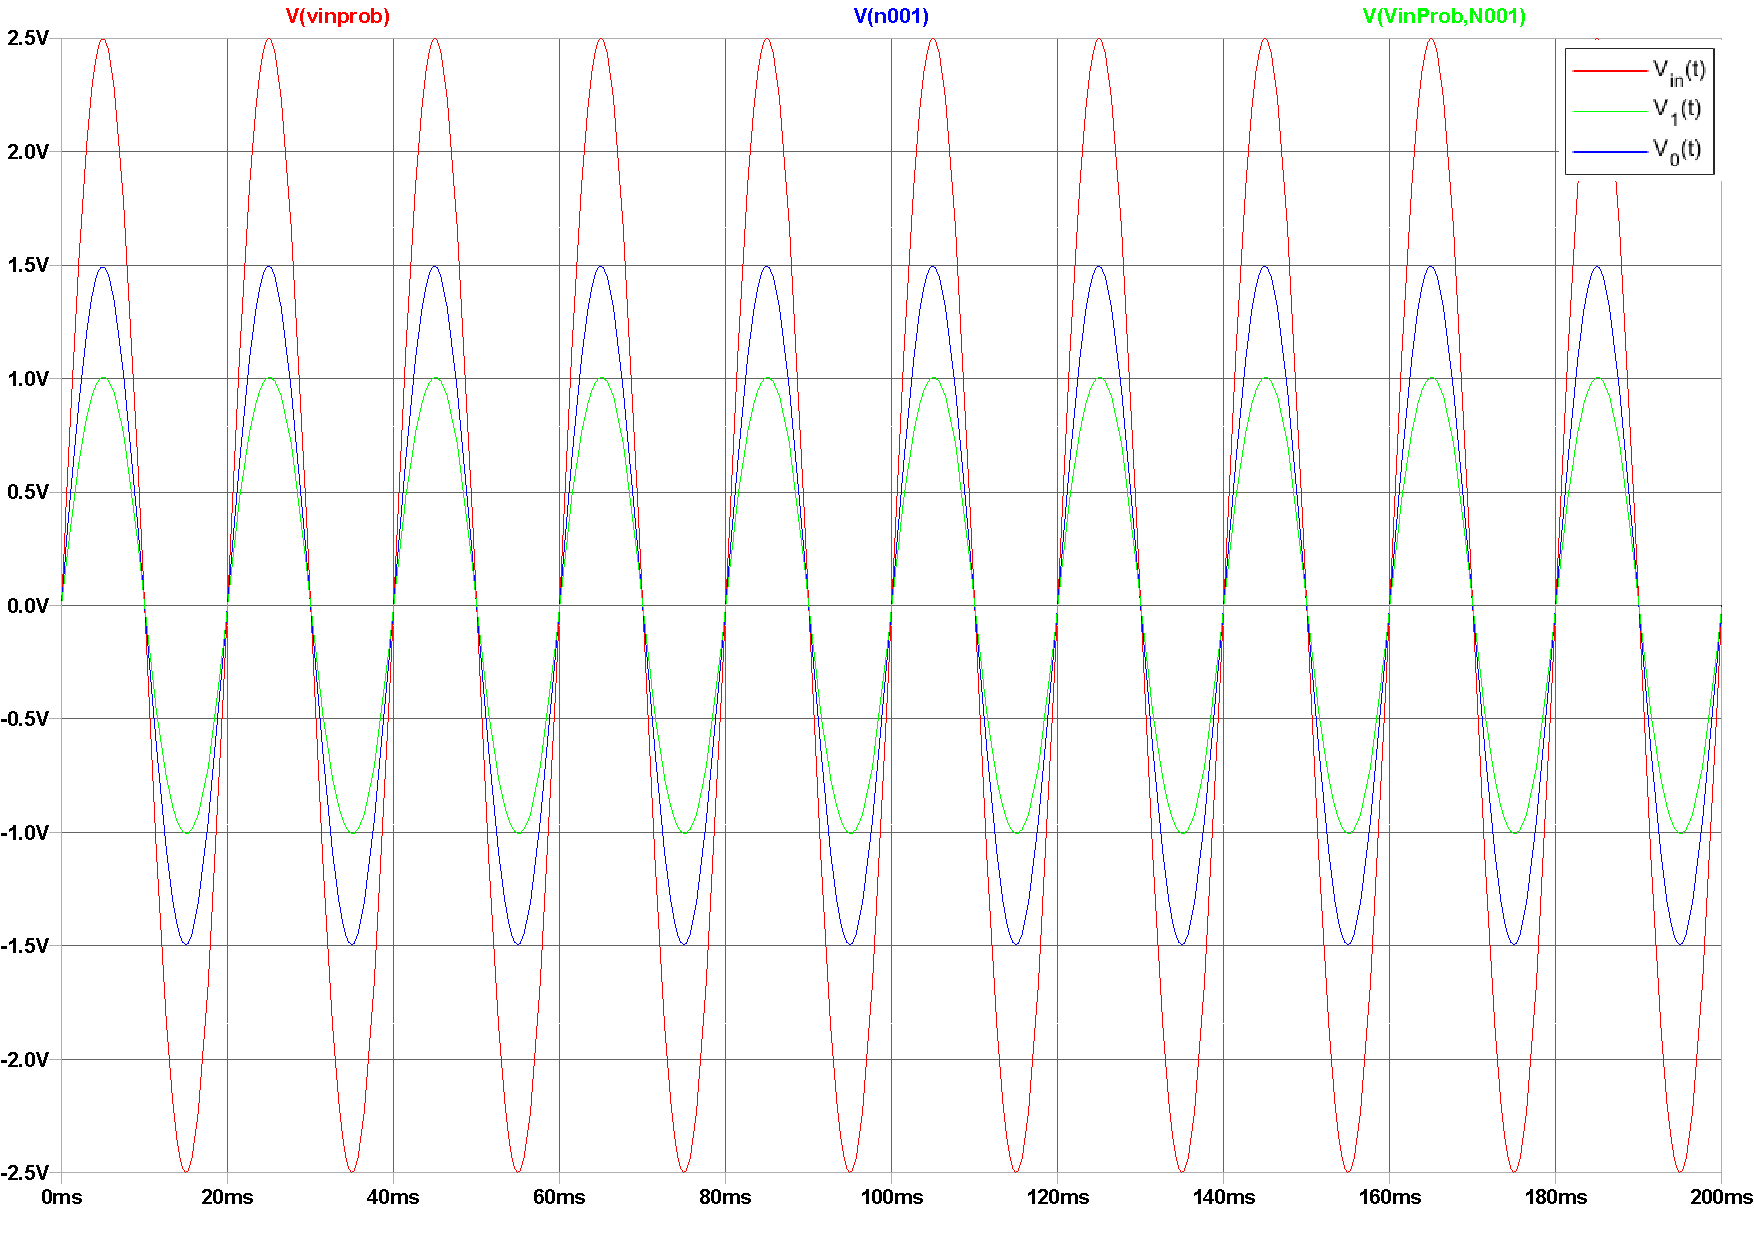
\includegraphics[scale=0.25]{2a_plot.pdf}}
		\caption{Experiment 2}
\end{figure}
	
https://components101.com/sites/default/files/component_datasheet/LDR\%20Datasheet.pdf \\

https://imagine.gsfc.nasa.gov/features/yba/M31_velocity/lightcurve/more.html \\

https://www.analog.com/en/applications/technology/3d-time-of-flight.html \\

https://www.ti.com/lit/an/sbau305b/sbau305b.pdf \\